% !TEX root = ../ausarbeitung.tex

\chapter{Entwicklung der Anwendung}

Im Rahmen der Masterarbeit wurde die beschriebende Web Applikation prototypisch entwickelt. Die dazu nötige Planung und die verwendeten Technologien wurden in den vorherigen Kapiteln geschildert. Nun wird auf den Prozess der Entwicklung und auf die detaillierte Struktur der Applikation eingegangen.\\

Das Entwicklung des Systems wurde in drei Teilprojekte untergliedert:
\begin{enumerate}
	\item Erstellung der Basisdatenbank aus dem Wörterbuch CELEX2
	\item Entwicklung des Backends mit python
	\item Entwicklund des Frontends mit gängigen Webtechnologien und AngularDart
\end{enumerate}

Dabei wurde Schritt 1 als Erstes durchgeführt, die Verfügbarkeit der Basisdatenbank war Voraussetzung um mit der Entwicklung von Front- und Backend zu beginnen. Als eine erste Version der Datenbank vorlag, wurde zunächst mit der Entwicklung eines minimalen Backends begonnen, welches die Kernfunktionalität - das Analysieren von Texten - beherrschte. Damit konnte eine erste Version des Frontends erstellt werden, um einen ersten Eindruck zu bekommen, wie alle Technologien miteinander funktionieren.\\
Im Anschluss konnten Front- und Backend parallel entwickelt werden. Es wurden immer wieder Funktionen im Backend entwickelt, woraufhin das Frontend angepasst wurde, um dem Nutzer diese Funktionen anzubieten. Zu diesem Zeitpunkt wurde auch die Basisdatenbank einige male überarbeitet, so ist das Gesamtsystem Schritt für Schritt auf eine agile Weise \tocite{agil} gewachsen. Im Folgenden wird näher auf die drei Teilprojekte eingegangen.

\section{Erstellung einer Basisdatenbank}
\label{sec:worddatabase}

Für die Segmentierung von Wörtern in Silben mit Betonung wird eine sqlite Datenbank verwendet, deren Entwicklung hier beschrieben wird. Als Grundlage für die Datenbank dient das digitale Lexikon \todo{Lexikon/woerterbuch...?} CELEX2, wie in Kapitel \toref{CELEX} beschrieben. Folgende Informationen wurden dem CELEX entnommen und in der Datenbank gespeichert:

\paragraph{Worttext}
Hier wurde darauf geachtet, eine einheitliche orthographische Form der Wörter durchzusetzen. Wörter bestehen nur aus Kleinbuchstaben (auch die Anfänge von Nomen und Eigennamen). Außerdem wird hier auf Umlaute verzichtet, \qq{ä} wird durch \qq{ae} ersetzt, \qq{ö} durch \qq{oe}, \qq{ü} durch \qq{ue} und \qq{ß} durch \qq{ss}. Beispielsweise wird das Wort \textit{Häuser} zu \textit{haeuser}. So kann beim Nachschlagen garantiert werden, dass ein Wort nicht wegen uneinheitlicher Schreibweise nicht gefunden wird, sofern alle Umlaute vorher ersetzt wurden.

\paragraph{Wortart}
Um Doppeldeutigkeit zu vermeiden wird ein Eintrag nur eindeutig über das Paar aus Worttext und Wortart identifiziert. Viele Grundformen von Verben kommen zum Beispiel auch als Nomen vor, werden aber dann groß geschrieben (\qq{sie sollte die Maschine \textit{verwenden}} gegen \qq{das \textit{Verwenden} der Maschine}). Die Bezeichner für Wortart sind in verschiedenen Systemen wie dem CELEX und dem NLP parser \textit{spacy} unterschiedlich, daher wird hier eine eigene - im Gesamtsystem konsistente - Benennung der Wortart eingeführt (die Benennung orientiert sich an den Tag Namen des spacy parsers, verwendet jedoch zur Unterscheidung Klein- statt Großschreibung):
\begin{itemize}
	\item Nomen: \qq{noun}
	\item Eigenname: \qq{propn}
	\item Verb: \qq{verb}
	\item Hilfsverb: \qq{aux}
	\item Adjektiv: \qq{adj}
	\item Adverb: \qq{adv}
	\item Artikel: \qq{det}
	\item Adposition (Überbegriff für Präposition und Postposition): \qq{adp}
	\item Pronomen: \qq{propn}
	\item Konjunktion: \qq{conj}
	\item Zahl: \qq{num}
	\item Partikel: \qq{part}
	\item Zahl: \qq{num}
\end{itemize}

\paragraph{Silbentrennung}
Die Silbentrennung enthält die einzelnen Silben, getrennt durch einen Querstrich (\qq{-}). Im Gegensatz zum Worttext erhält dieser Eintrag Groß- und Kleinschreibung, sowie alle Umlaute. Die Silbentrennung des Wortes \textit{Möglichkeit} ist also \textit{Mög-lich-keit}.

\paragraph{Betonungsmuster}
Das Betonungsmuster identifiziert eine Silbe als Hauptbetonung im Wort. Dieser Eintrag ist ein String aus aneinandergereihten \qq{0} und \qq{1} Werten. Die \qq{1} bezeichnet dabei die betonte Silbe, die \qq{0} stellt eine unbetonte Silbe dar. Nebenbetonungen werden im Rahmen dieser Arbeit vernachlässigt. Das Betonungsmuster besteht nur aus einer einzigen \qq{1} - der Hauptbetonung - während alle anderen Silben unbetont (\qq{0}) bleiben. Beispiel resultiert das Wort \textit{hervorragend} mit der Silbentrennung \textit{her-vor-ra-gend} in das Betonungsmuster \qq{0100}.

\paragraph{Lemma}
was genau? auch im celex, keine wirkliche anwendung in der app, vielleicht ausblick

Neben den Worteinträgen sollen in der Datenbank noch Informationen über die Herkunft der Wörter gespeichert werden. Neben den Basiseinträgen, die aus dem CELEX extrahiert werden, wird den Nutzern später die Möglichkeit gegeben Einträge zur Datenbank hinzuzufügen. Um diesen Vorgang nachvollziehbar zu machen gibt es eine zweite Tabelle, in welcher Einträge für neu hinzugefügte Wörter mit Zeitstempel angelegt werden. Das Folgende Schema \ref{figure:worddatabase} zeigt die Struktur der Wortdatenbank.

\begin{figure}[h!]
	\centering
	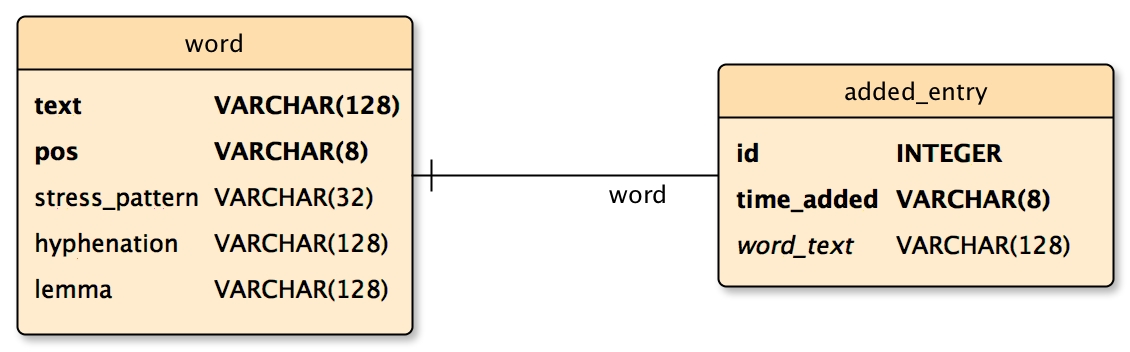
\includegraphics[width=.6\linewidth]{figures/worddb}
	\caption{Schema der Wortdatenbank (\textit{word.db})}
	\label{figure:worddatabase}
\end{figure}

Alle in der Worttabelle beschriebenen Einträge sind auch im CELEX vorhanden. Der Folgende Abschnitt beschreibt, wie die Daten aus dem Lexikon extrahiert und in der Wortdatenbank gespeichert wurden.

\subsection{Impementierung}

Für die Generierung der Datenbank wurde das python Projekt \textit{celex2db} erstellt, welches in \qq{/backend/celex2db} zu finden ist (alle Pfadangaben in diesem Abschnitt beziehen sich auf dieses Verzeichnis). Die Daten im CELEX \todo{in Forschungsstand teil verschieben} sind über mehrere Dateien verteilt. So gibt es eine Teilung in Sprachen (für die Datenbank werden nur Deutsche Wörter benutzt, zu finden in \qq{celex2/german}), Wörter und Lemmata sowie in Orthographie, Phonologie und Morphologie. Die Teilung in Wort und Lemma spart Speicherplatz. Das Lemma eines Verbs, zum Beispiel, ist die Grundform dieses. Zur Beugung \textit{gehst} gehört also das Lemma \textit{gehen}. Viele Eigenschaften des Verbs \textit{gehen} beziehen sich auf alle Beugungen \todo{=Flexionsformen?}, so müssen diese nicht für alle Verbformen redundant gespeichert werden.\\
Die Einträge in den Wortlisten des CELEX verweisen jeweils mit einer ID auf den zugehörigen Eintrag in der Lemma Liste. Da in der zu entwickelnden Datenbank auch das Lemma gespeichert werden soll, müssen sowohl Wort Listen als auch Lemma Listen geparsed werden.\\

Das Hauptskript \qq{celex2db.py} führt die folgenden Schritte aus:
\begin{enumerate}
	\item Parsen der orthographischen Lemma Liste
	\item Parsen der orthographischen und phonologischen Wort Listen
	\item Generierung von Einträgen aus Wort und Lemma Listen und Schreiben in die Datenbank
\end{enumerate}
Während der Ausführung des Skripts werden Schrittweise Fortschrittsangaben mit Fehlern ausgegeben (Schrittweite im Skript einstellbar), da das Parsen und Erstellen der Datenbank einige Zeit benötigt (mehr dazu im Abschnitt \toref{Ergebnisse}).

Die Klasse \texttt{CelexDictionary} im Skript \qq{celex.py} bietet die Methoden zum Parsen der Wort und Lemma Listen. Die Struktur ist in \toref{Figur} dargestellt.\\

\todo{Klassendiagramm CelexDictionary}

In der \texttt{parseLemma} Methode wird die CELEX Datei \qq{gml.cd} verarbeitet. Die morphologische Informationen zu den Lemmata enthält. Jede Zeile enthält ein Lemma, für welches in der Struktur \texttt{CelexLemma} die ID des Lemmas, Text und Wortart gespeichert werden.\\

In der \texttt{parseWords} Methode werden nun die beiden Dateien \qq{g\textbf{p}w.cd} und \qq{g\textbf{o}w.cd} verarbeitet, welche phonologische und orthographische Informationen zu allen enthaltenen Beugungen der Wörter enthalten. Die IDs und Reihenfolge in beiden Wortlisten stimmen überein, sodass beide Listen gleichzeitig verarbeitet werden können. Aus der phonologischen Liste werden der Text des Wortes, der Verweis auf das zugehörige Lemma (lemma\_id) sowie die phonologische Darstellung entnommen. Die orthographischen Liste liefert lediglich die Silbentrennung.\\
Danach wird in der zuvor verarbeiteten Liste der Lemmas, mithilfe der \texttt{lemma\_id} der Text passende Lemmas gesucht und alle verfügbaren Daten in der Struktur \texttt{CelexWord} gespeichert. Die Hauptklasse \texttt{CelexDictionary} enthält ein python Dictionary aller \texttt{CelexWord} Einträge, siehe \toref{klassendiagram figur}.

Letztendlich werden die Einträge der Wortliste im Skript \qq{writeSQLite.py} in die Datenbank übertragen. In einem frühen Entwicklungsstadium wurden hier SQL Instruktionen verwendet um die Datenbankeinträge zu erstellen. Nach der Entwicklung des \texttt{DictionaryService} im Backend (genauer beschrieben im Abschnitt \toref{DictionaryService}) wurde später direkt auf diesen zugegriffen, um Redundanten Code zu vermeiden. Ein einfacher Funktionsaufruf der Methode \texttt{add\_word} des \texttt{DictionaryService} fügt den Eintrag der Wortdatenbank hinzu.

\subsection{Ergebnisse}

Ein Wort soll eindeutig identifizierbar sein durch den Worttext und die Wortart. Daher wurde in der Datenbank die Kombination der Felder \textit{text} und \textit{pos} (part of speech/Wortart) als Primärschlüssel gewählt. Ein doppeltes Einfügen eines Wortes in die Datenbank verletzt den SQL \textit{UNIQUE Constraint}, und ist somit nicht möglich. Die dadurch von python geworfene Exception wird in diesem Fall abgefangen und und die \texttt{add\_word} Methode liefert \texttt{None} zurück.\\
Trotz der Wortidentifizierung anhand von zwei Merkmalen, beinhaltet der CELEX teilweise redundante Informationen. 4 356 Einträge verursachen aufgrund des \textit{UNIQUE Constraint} Fehler, da sie mit gleichem Text und gleicher Wortart schon in der Datenbank waren, diese wurden somit übersprungen. Bei einem kompletten Neuaufbau der Datenbank aus dem CELEX werden 360 243 Wörter hinzugefügt. Die Datenbank wurde als sqlite Datei \qq{/backend/db/words.db} angelegt.

\section{Backend}

Das in python mit dem Web-Framework flask entwickelte Backend verarbeitet sämtliche, vom Frontend gesendeten HTTP requests. Es sendet entweder eine Antwort mit den geforderten Daten oder einen HTTP Fehlercode mit Fehlermeldung. Das Backend Projekt befindet sich in \qq{/backend/API}. Es wurde in die drei Services \textit{DictionaryService}, \textit{UserService} und \textit{VerificationService} strukturiert. Das Hauptsript \todo{rename} \qq{LinguisticTextAnnotation.py} verwaltet diese Services, startet die flask Applikation und definiert die einzelnen Routen für HTTP requests (diese werden im folgenden Abschnitt aufgelistet). Folgende Grafik zeigt eine Übersicht über die Struktur des Backends.

\todo{Grafik Backend}

\subsection{HTTP Routen}
Tabelle \ref{table:backendroutes} bietet eine Übersicht über die verfügbaren Routen, welche die HTTP requests verarbeiten. Zudem werden kurz der Zweck und die Parameter der Route beschrieben. Ein \textit{X} in der Spalte Authentifizierung bedeutet, dass die Mail Adresse und das Passwort des Nutzers übergeben werden muss. Diese werden nicht extra in der Spalte Parameter aufgeführt (außer in der \qq{/user/authenticate} Route, diese dient ausschließlich dazu, die Übermittelten Nutzer Credentials zu prüfen).
\todo{include return JSON fields...}

\begin{table}[h!]
	\centering
	\begin{tabular}{|l|l|l|c|}
		\hline
		\textbf{Route} & \textbf{Parameter} & \textbf{Methode} & \textbf{Auth.}\\
		\hline
		\hline
		/query/word & text, pos & GET & \\
		\hline
		/query/text & text & POST & \\
		\hline
		/query/segmentation& word & GET & \\
		\hline
		\hline
		/user/register & email, password, & POST & \\
		& first\_name, last\_name, is\_expert &&\\
		\hline
		/user/authenticate & \textit{email, password} & POST & X\\
		\hline
		/user/list & \todo{remove} & GET & \\
		\hline
		/user/delete & \todo{implement} & POST & X\\
		\hline
		\hline
		/user/word/add& text, stress\_pattern, hyphenation, pos & POST & X\\
		\hline
		/user/word/delete& id & POST & X\\
		\hline
		/user/word/list & - & POST & X\\
		\hline
		\hline
		/user/configuration/add & name, \textit{options} & POST & X\\
		\hline
		/user/configuration/update & id, name, \textit{options}  & POST & X\\
		\hline
		/user/configuration/list & - & POST & X\\
		\hline
		/user/configuration/delete & id & POST & X\\
		\hline
		\hline
		/user/text/add & title, text & POST & X\\
		\hline
		/user/text/delete & id & POST & X\\
		\hline
		/user/text/list & - & POST & X\\
		\hline
		\hline
		/user/verification/query & - & POST & X\\
		\hline
		/user/verification/submit & id, stress\_pattern, hyphenation & POST & X\\
		\hline
	\end{tabular}
	\caption{Backend routen für HTTP requests mit Parametern und Methode}
	\label{table:backendroutes}
\end{table}

Die bei \qq{user/configuration/} nicht aufgeführten \textit{options} bestehen aus allen für die Annotationsvorlage gespeicherten einstellungen. Dies sind die Folgenden Felder: \textit{stressed\_color, unstressed\_color, word\_background, alternate\_color, syllable\_separator, line\_height, word\_distance, syllable\_distance, font\_size, letter\_spacing, use\_background, highlight\_foreground, stressed\_bold, use\_alternate\_color, use\_syllable\_separator, part\_of\_speech\_configuration}.

\subsection{Dictionary Service}

Das Modul \textit{DictionaryService.py} verarbeitet Anfragen zur Textanalyse, verwaltet die Wortdatenbank und generiert Vorschläge für die manuelle Segmentierung von Wörtern \todo{Segmentierung beschreiben}. Das Schema der Wortdatenbank zeigt Figur \ref{figure:worddatabase}. Folgende Klassen werden definiert:
\begin{itemize}
	\item \texttt{Word}: Entspricht Tabelle \textit{word} in der Wortdatenbank und speichert die Merkmale eines Wortes.
	\item \texttt{AddedEntry}: Enthält einen Verweis (Fremdschlüssel) auf ein hinzugefügtes Wort und dessen Erstellungszeitpunkt.
	\item \texttt{Segmentation}: Modelliert einen Segmentierungsvorschlag. Die Klasse enthält Worttext, Segmentierung und Betonungsmuster. Außerdem speichert sie den Namen (\texttt{origin}) und die Herkunft (\texttt{source}) der Quelle des Vorschlags (z.B. MARY TTS).
\end{itemize}

Im Folgenden werden die Funktionen des \textit{DictionaryService} genauer beschrieben.

\subsubsection{Funktionen der Wortdatenbank}
\begin{itemize}
	\item Die Methode \texttt{add\_word} bekommt Worttext, Betonungsmuster, Wortteilung, Lemma und Wortart übergeben (s. Abschnitt \ref{sec:worddatabase}), fügt das Wort der Datenbank hinzu und liefert eine \texttt{Word} Instanz zurück. Im Falle eines Fehlers oder falls das Wort schon existiert, gibt die Methode \texttt{None} zurück.
	
	\item \texttt{query\_word} schlägt ein Wort mit den Parametern Worttext und Wortart in der Datenbank nach und gibt das annotierte Wort im JSON (\textit{text}, \textit{stress\_pattern}, \textit{hyphenation}, \textit{lemma}, \textit{pos}) Format zurück. Als Parameter kann optional der eingeloggte Nutzer übergeben werden. Ist das der Fall, wird zuerst überprüft, ob im Nutzeraccount (s. Abschnitt \ref{sec:userservice}) eine manuelle Segmentierung für das Wort gespeichert ist und falls ja, diese zurückgegeben. Werden in der Wortdatenbank mehrere Wörter gefunden, die dem gesuchten Worttext entsprechen, wird zusätzlich die Wortart geprüft und der passende Eintrag (bzw. der Erste Eintrag, falls kein Wort mit der entsprechenden Wortart gefunden wird) zurückgegeben.
	
\subsubsection{Textanalyse}
Die Methode \texttt{query\_text} bekommt den gesamten zu analysierenden Text übergeben (sowie optional den eingeloggten Nutzer für manuelle Worteinträge). Der Text wird zunächst mit dem spacy Parser analysiert. Dieser zerlegt den Text in einzelne Wörter und Trennzeichen und gibt eine Liste von Tokens zurück. Nun wird über die Liste der Tokens iteriert und dabei wiederum eine Liste von JSON Einträgen generiert, welche am Schluss von der Methode zurückgegeben wird. Jedes spacy Token liefert den Worttext \texttt{text} die Wortart \texttt{pos\_} und das Lemma \texttt{lemma\_}. Das Token wird wie folgt verarbeitet:

\begin{enumerate}
	\item In jedem Fall wird ein neuer JSON Eintrag angelegt und die Felder \texttt{text}, \texttt{pos} und \texttt{lemma} mit den entsprechenden Inhalt des spacy Tokens gefüllt.
	
	\item Enthält der Worttext einen Linebreak \qq{\texttt{\textbackslash n}}, so wird das JSON Feld \texttt{type} mit \textit{linebreak} belegt.
	
	\item Enthält der Worttext einen Trennstrich \qq{\texttt{-}}, so handelt es sich um ein zusammengesetztes Wort (z.B. \textit{100-Millionen-Einwohner-Staat}). Hier werden alle Trennstriche durch Leerzeichen ersetzt. Der resultierende String wird dann erneut mit spacy analysiert und die Tokens dann entsprechend verarbeitet. Hinter jedem Teilwort (außer dem Letzten) wird manuell der Trennstrich als eigenes Token eingefügt.
	
	\item Entspricht der Wortart-Tag einem String aus \texttt{['X',} \texttt{'PUNCT', }\texttt{'NUM', }\\
	\texttt{'SPACE']}, so handelt es sich um eine dem Parser unbekannte Zeichenfolge, eine Zahl, ein Satz- oder Leerzeichen. Diese Tags werden nicht nachgeschlagen sondern mit dem JSON \texttt{type} Feld \textit{ignored} der Rückgabeliste hinzugefügt.
	
	\item Trifft keiner dieser Sonderfälle zu, wird das Wort mit der Methode \texttt{query\_word} nachgeschlagen. Wird dieses gefunden (Rückgabewert nicht \texttt{None}), wird der \texttt{type} auf \textit{annotated\_word} gesetzt. Das JSON Feld \texttt{annotation} enthält dann die Informationen des annotierten Wortes (von \texttt{query\_word} zurückgegeben). Ist das Wort nicht in der Datenbank, so enthält das Feld \texttt{type} den Wert \textit{not\_found}.
\end{enumerate}

\end{itemize}

\subsubsection{Generierung von Segmentierungsvorschlägen}
\todo{pyphen, MARY...}

\subsection{User Service}
\label{sec:userservice}

was macht dieser?\\
sqlite Tabellen\\

\begin{figure}[h!]
	\centering
	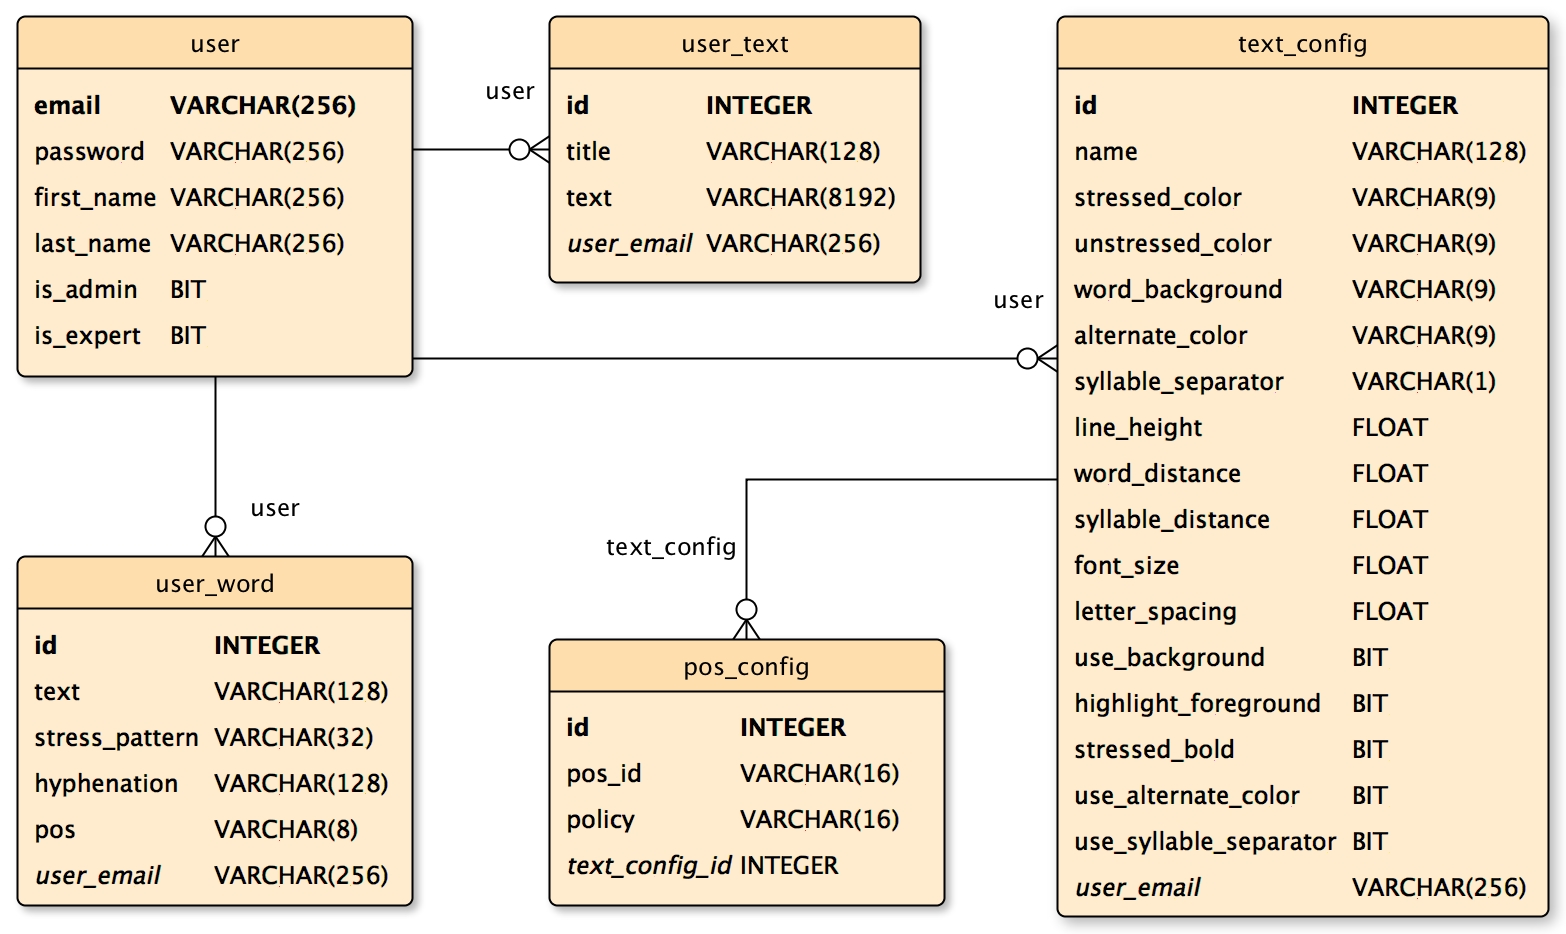
\includegraphics[width=.8\linewidth]{figures/userservicedb}
	\caption{Schema der User Datenbank (\textit{user.db})}
	\label{fig:userdb}
\end{figure}

Klassendiagramme\\

\subsection{Verification Service}
was macht dieser?\\
sqlite Tabellen\\
Klassendiagramme\\


\section{Frontend}

angular dart app\\
komponenten s. software stack erklärung\\

app\_component, providers, directives\\

\subsection{Datenmodell}
word, syllable, klassendiagramme, interaktion...

\subsection{Begrüßungsseite}

home\_component\\
angular router links

\begin{figure}[h!]
	\centering
	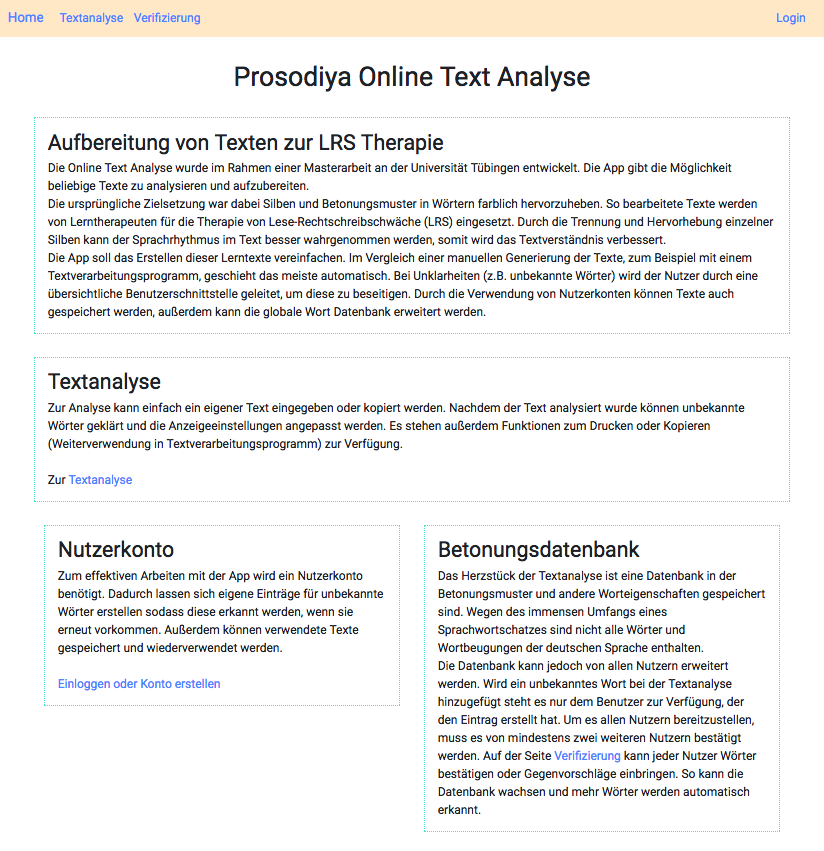
\includegraphics[width=.6\linewidth, frame]{figures/frontend/home}
	\caption{Bildschirmfoto der Begrüßungsseite}
	\label{fig:frontend-home}
\end{figure}

\subsection{Text Analyse}

ui und service

\begin{figure}[h!]
	\centering
	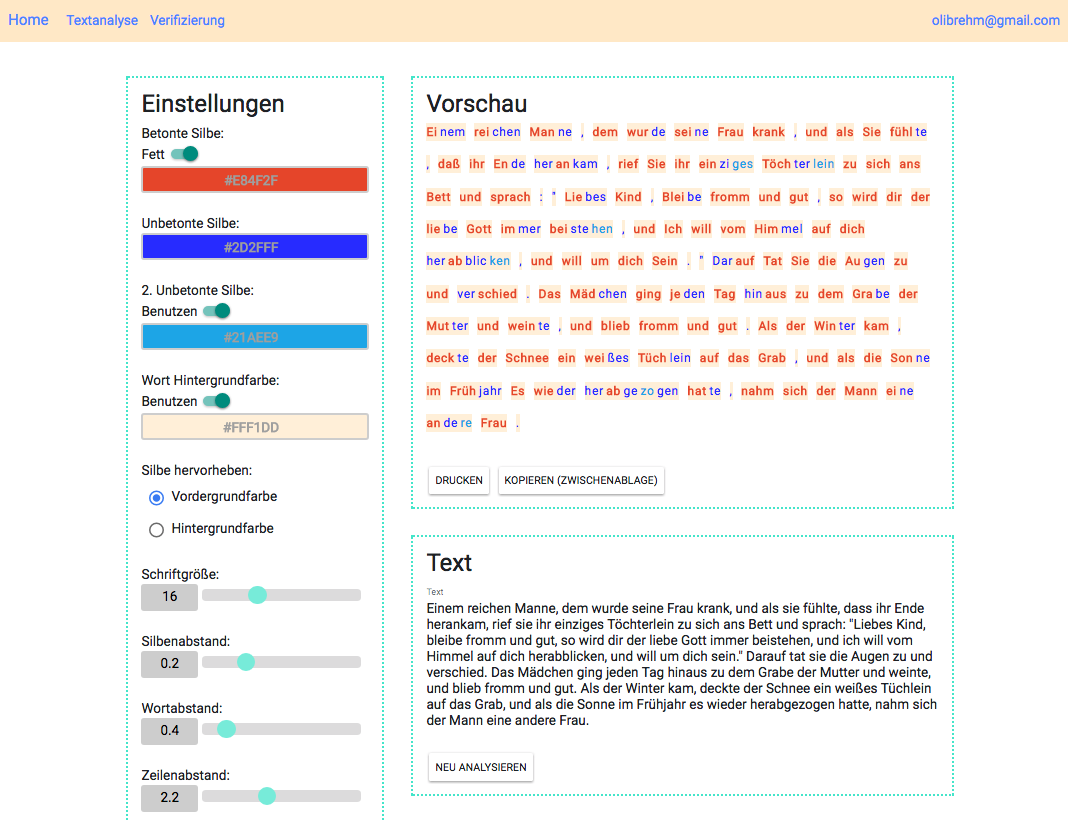
\includegraphics[width=.8\linewidth, frame]{figures/frontend/textanalyse}
	\caption{Bildschirmfoto der Textanalyse}
	\label{fig:frontend-textanalyse}
\end{figure}

\subsubsection{TextAnalysisService}

funktionen, model abhängigkeiten

\subsubsection{Texteingabe}

texteingabe, material-input\\

\subsubsection{Textvorschau}

iterieren über wörter\\
span je nach word state\\
notfound wörter mit link zu word review\\
linebreaks (sind wörter, spezieller state)\\

editierbare wörter, css aus komponente\\
popup:\\
\begin{itemize}
	\item annotieren oder nicht
	\item manuelles Betonungsmuster
	\item manuelle Silbentrennung
	\item gleiche wörter übernehmen
	\item Wortart
	\item Lemma
\end{itemize}

\begin{figure}[h!]
	\centering
	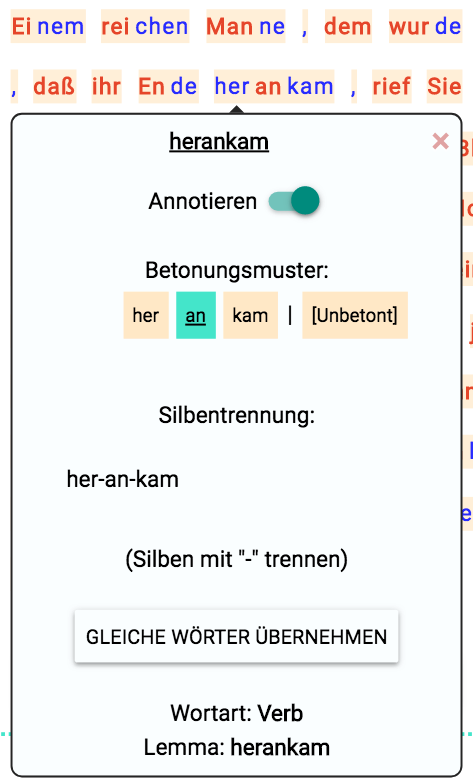
\includegraphics[width=.4\linewidth, frame]{figures/frontend/wordpopup}
	\caption{Bildschirmfoto der spezifischen Worteinstellungen}
	\label{fig:frontend-wordconf}
\end{figure}

span für silben\\
style aus komponente\\
separator zeichen\\

drucken, css vorlage, @media\\
text kopieren, js/dart magic\\

\subsubsection{Textoptionen}

text neu analysieren\\
text speichern, mit titel\\
neuen text eingeben

\subsection{Annotationseinstellungen}

verschiedene einstellungen\\
in server für user gespeichert\\

\subsubsection{TextConfigurationService}

TODO refactor, diesen service neben user service anlegen

\subsubsection{User Interfache für Einstellungen}
betonte silbe\\
fett, farbe\\

color picker\\

unbetonte silben\\
farbe\\
2. farbe, benutzen\\

\begin{figure}[h!]
	\centering
	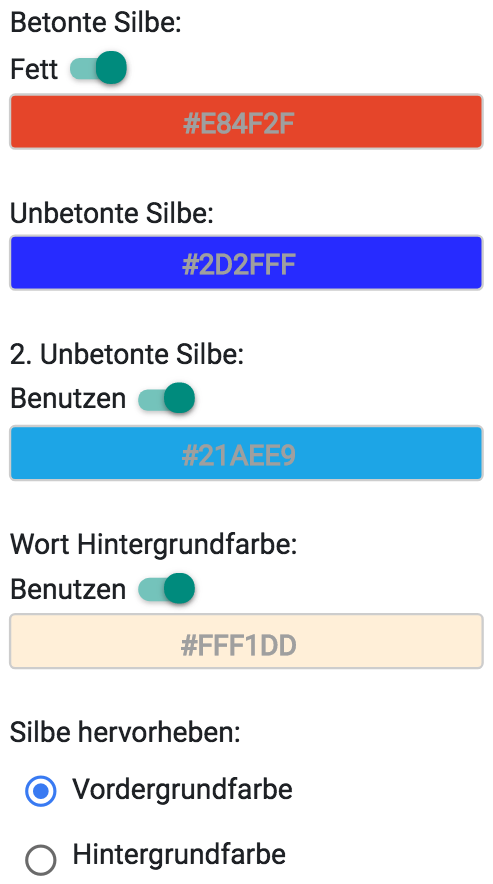
\includegraphics[width=.4\linewidth, frame]{figures/frontend/config-color}
	\caption{Bildschirmfoto der Farbeinstellungen}
	\label{fig:frontend-colorconf}
\end{figure}

worthintergrund, warum, in welcher einstellung sinnvoll?

größen und abstände\\
\begin{itemize}
	\item Schriftgröße
	\item Silbenabstand
	\item Wortabstand
	\item Zeilenabstand
	\item Zeichenabstand
\end{itemize}

\begin{figure}[h!]
	\centering
	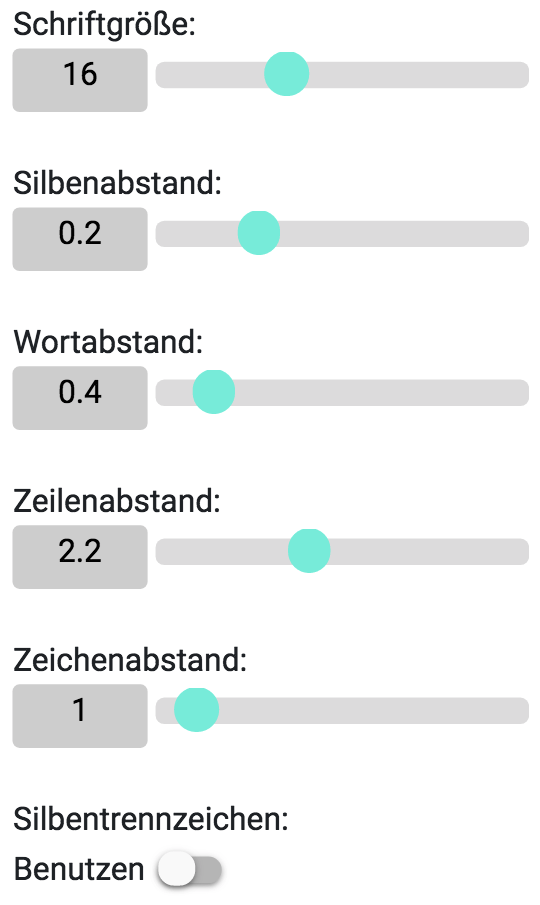
\includegraphics[width=.4\linewidth, frame]{figures/frontend/config-text}
	\caption{Bildschirmfoto der Texteinstellungen}
	\label{fig:frontend-textconf}
\end{figure}

custom slider\\

Silbentrennzeichen\\
warum, benutzen, eingabe\\

Wortart dropdown\\
funktionen separat wür die verschiedenen Wortarten\\
dropdown\\
funktion iteriert über alle wörter im text und wendet eigenschaft auf jedes passende Wort an\\
funktionen:\\
\begin{itemize}
	\item Annotieren
	\item Unbetont
	\item Ignorieren
\end{itemize}

\begin{figure}[h!]
	\centering
	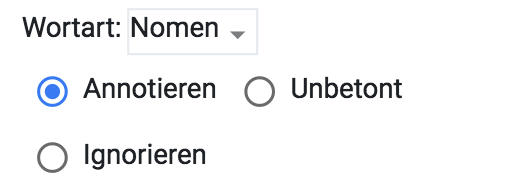
\includegraphics[width=.4\linewidth, frame]{figures/frontend/config-pos}
	\caption{Bildschirmfoto der spezifischen Wortart Einstellungen}
	\label{fig:frontend-pos-einstellungen}
\end{figure}

\subsubsection{Annotationsvorlagen}

speichert alles\\
name der vorlage\\
liste, aktivieren, löschen\\
neue vorlage anlegen oder momentane speichern\\

\begin{figure}[h!]
	\centering
	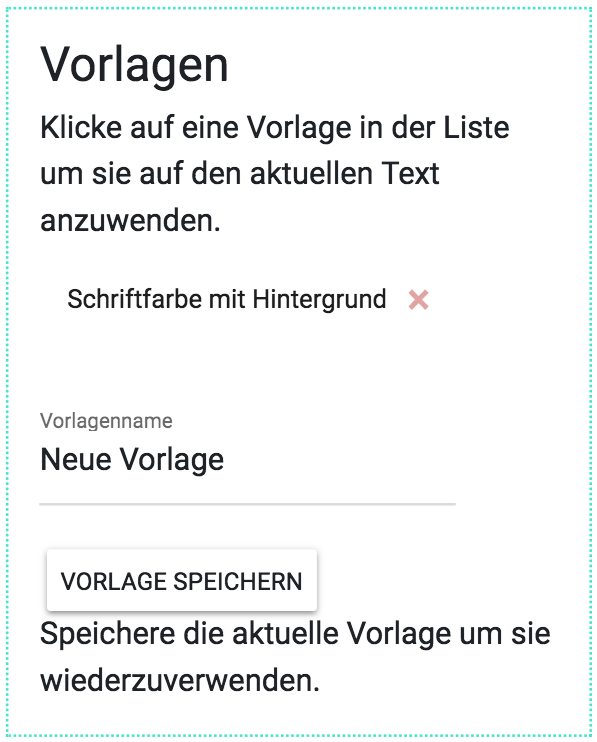
\includegraphics[width=.4\linewidth]{figures/frontend/config-vorlagen}
	\caption{Bildschirmfoto der UI zur Verwaltung und Verwendung von Annotationsvorlagen}
	\label{fig:frontend-vorlagen}
\end{figure}

\subsection{Manuelle Wortanalyse}

TBD
\begin{figure}[h!]
	\centering
	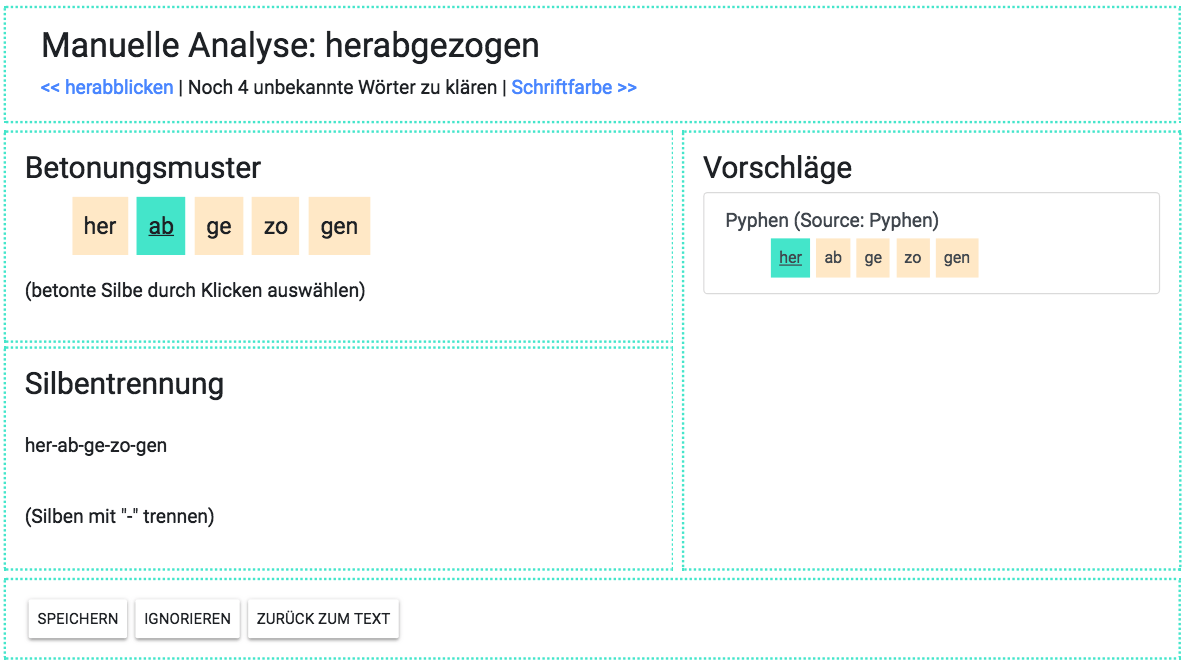
\includegraphics[width=.8\linewidth]{figures/frontend/manuelle-analyse}
	\caption{Bildschirmfoto der Manuellen Wortanalyse\todo{bild wo MARY funktioniert!}}
	\label{fig:frontend-manuelle-analyse}
\end{figure}

\subsection{Nutzerkonto}

TBD
\begin{figure}[h!]
	\centering
	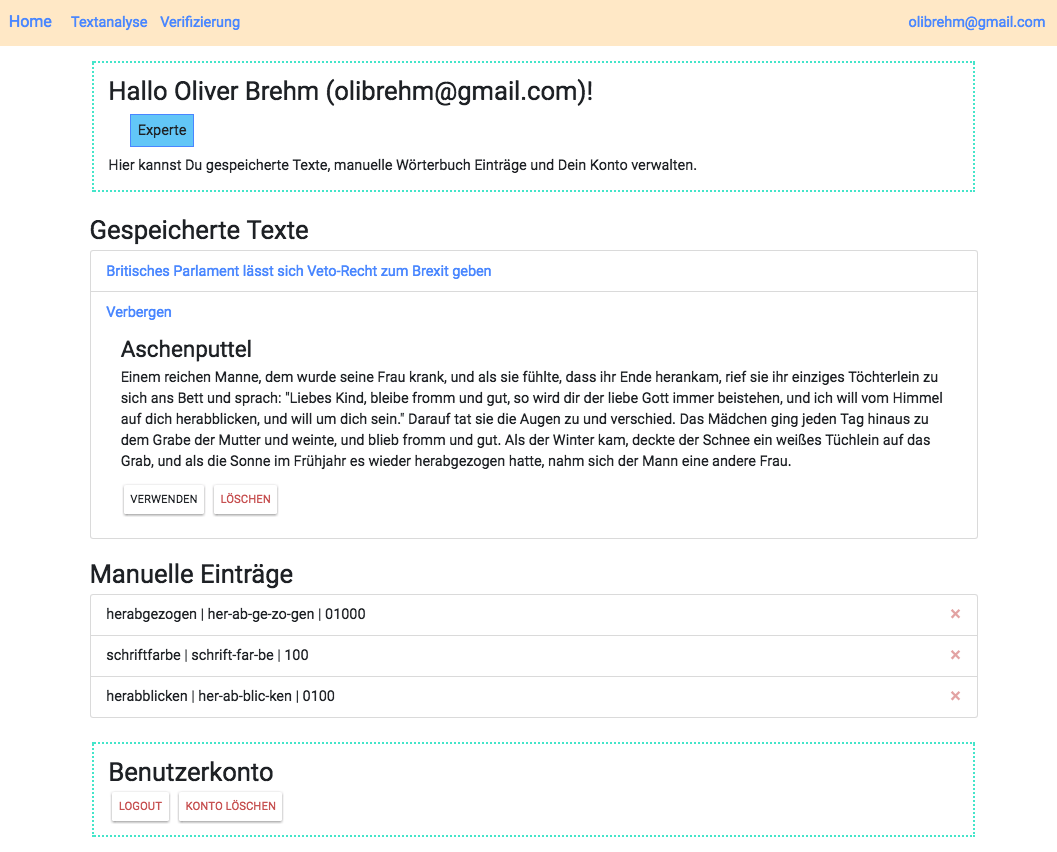
\includegraphics[width=.8\linewidth, frame]{figures/frontend/user-account}
	\caption{Bildschirmfoto der Nutzerkontoseite}
	\label{fig:frontend-useraccount}
\end{figure}

\subsection{Wort Verifizierung}

TBD
\begin{figure}[h!]
	\centering
	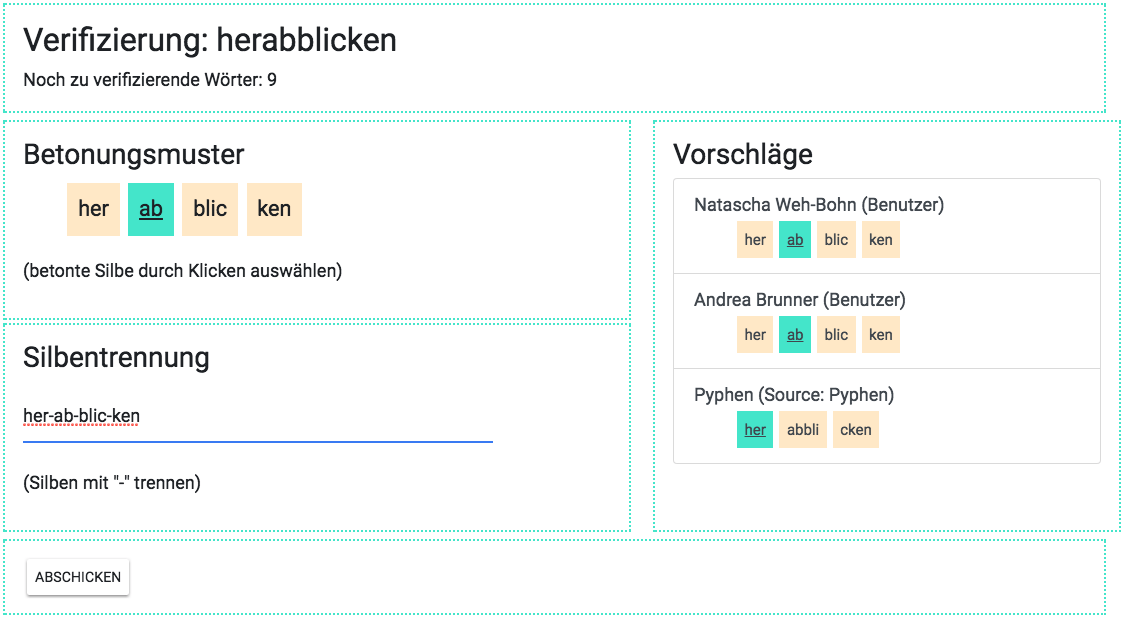
\includegraphics[width=.8\linewidth]{figures/frontend/verifizierung}
	\caption{Bildschirmfoto der Verifikation von manuell hinzugefügten Wörtern}
	\label{fig:frontend-verification}
\end{figure}